% @Author: Taha Bouhsine


%%%%%%%%%%%%%%%%%%%%%%%%%%%%
% CHAPTER                  %
%%%%%%%%%%%%%%%%%%%%%%%%%%%%
\setcounter{mtc}{10}

\chapter{Technical And Environmental Study}%
\label{chap:chapter_tree}
\minitoc
\section{Capture of technical needs}
The capture of technical needs identifies all the constraints and the choices dimensioning the design of the system.

The tools and materials selected as well as the management of integration constraints generally conditioning the prerequisites of general architecture.

The capture of technical needs is as follows:
\begin{itemize}\addtolength{\itemsep}{-0.35\baselineskip}
      \item
            Capturing software specifications.

      \item
            Capturing specifications related to hardware configuration.

\end{itemize}

\subsection{Capturing Software Specifications}
These are technical features that the system will provide to the user regardless of the business or functional term.

We will, therefore, list a list of technical functionalities that our system will be able to provide and offer to users, which is why we have introduced the concepts of operator and technical use cases:

\paragraph{Technical actors}
Also called "technical actors" of the system, these are the actors who benefit from the technical functionalities of the system:
\begin{itemize}\addtolength{\itemsep}{-0.35\baselineskip}
      \item
            User: These are the people who use the system functionality in one way or another.
      \item
            Administrator: this is the person responsible for managing all the management of the platform as well as that of the users.
\end{itemize}

\paragraph{Identification of technical use cases}

\begin{longtable}{|m{10em}|m{10em}|m{10em}|}\hline
  Aspects    &                  Use Cases                       & Sub-Use Cases                                       \\\hline

      \multirow{4}{*}{Security management} & \multirow{5}{*}{Authentication}          & Register                                                    \\\cline{3-3}
                                           &                                          & Login                                                       \\\cline{3-3}
                                           &                                          & Reset Password                                              \\\cline{3-3}
                                           &                                          & Change password                                             \\\cline{3-3}
                                           &                                          & Logout                                                      \\\cline{2-3}
                                           & \multirow{1}{*}{Confidentiality}         & Role management                                             \\\cline{2-3}
                                           & \multirow{2}{*}{Secure payment}          & Send Payment                                                \\\cline{3-3}
                                           &                                          & Receive Payment                                             \\\cline{2-3}
                                           & \multirow{2}{*}{Backup and restore}      & Save the database                                           \\\cline{3-3}
                                           &                                          & Restore the database                                       \\\hline
      \multirow{7}{*}{Data managment}      & \multirow{1}{*}{Dynamic data}            & Dynamic data dispaly                                       \\\cline{2-3}
                                           & \multirow{1}{*}{Integrity}               & Simultaneous updates                                       \\\cline{2-3}
                                           & \multirow{1}{*}{Interoperability}        & Network deployment                                         \\\cline{2-3}
                                           & \multirow{1}{*}{Compatibility}           & Run on different browsers and platforms                    \\\cline{2-3}
                                           & \multirow{2}{*}{History}                 & Get all the user created projects fundraised               \\\cline{3-3}
                                           &                                          & Get all the user created projects fundraised               \\\cline{2-3}
                                           & \multirow{1}{*}{Statistics}              & Display platform statistics                                \\\cline{2-3}
                                           & \multirow{1}{*}{Fund}                    & Fund migration from anonymous user                         \\\hline
      \multirow{4}{*}{Help management}     & \multirow{2}{*}{Gestion des erreurs}     & Logging Viewing types of errors                            \\\cline{3-3}
                                           &                                          & Send the error by email to the administrator               \\\cline{2-3}
                                           & \multirow{1}{*}{Aide en ligne}           & Consult the user help Guide                                \\\cline{2-3}
                                           & \multirow{1}{*}{Notifications}           & Confirmation or error message                              \\\cline{2-3}
                                           & \multirow{1}{*}{Mails}                   & Sending emails                                             \\\hline
      \multirow{2}{*}{Payment management}  & \multirow{1}{*}{Multi-currency platform} & Choose a currency for purchase and payment                 \\\cline{2-3}
                                           & \multirow{1}{*}{Payment method}          & Possibility to choose a payment method                     \\\hline
      \multirow{3}{*}{Optimization}        & \multirow{1}{*}{Navigation}              & Nested operations                                          \\\cline{2-3}
                                           & \multirow{1}{*}{Sharing}                 & Possibility to share your donation                         \\\cline{2-3}
                                           & \multirow{1}{*}{Theming}                 & Possibility to switch themes between dark and light themes \\\hline

      \caption{Identification of technical objectives and use cases}
      \label{tab:id_tech_objec_uc}
\end{longtable}

% \paragraph{ Technical description use cases }
% View all the use cases described in the appendix \ref{sec:ucd}




\section{Adopted Software Architecture}
% TODO Link the architectures
The software architecture of a system describes its major components, their relationships, and how they interact with each other.

It essentially serves as a blueprint. It provides an abstraction to manage the system complexity and establish communication and coordination among components.

It helps us to determine how we should handle the codebase of our application, the technology to go with, and what cloud architecture is best for our application.

\begin{figure}[!ht]
      \center
      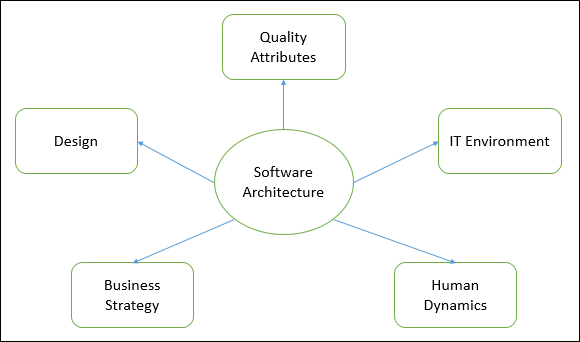
\includegraphics[scale=0.70]{assets/software_arch.jpg}
      \caption{Software Architecture Factors}
      \label{fig:mvc}
\end{figure}

\subsection{Software Architecture Pattern}

The Model View Controller \ac{MVC} design pattern specifies that an application consists of a data model, presentation information, and control information. The pattern requires that each of these be separated into different objects.

% MVC is more of an architectural pattern, but not for a complete application. MVC mostly relates to the \ac{UI} / interaction layer of an application. We’re still going to need a business logic layer, maybe some service layer and data access layer.
The MVC architecture is a software architectural pattern in which the application logic is divided into three components on the basis of functionality. These components are called: Models - represent how data is stored in the database Views - the components that are visible to the user, such as an output or a GUI Controllers, the components that act as an interface between models and views

% \begin{enumerate}
%       \item Model contains only the pure application data, it contains no logic describing how to present the data to a user.
%       \item View presents the model’s data to the user. The view knows how to access the model’s data, but it does not know what this data means or what the user can do to manipulate it.
%       \item Controller exists between the view and the model. It listens to events triggered by the view (or another external source) and executes the appropriate reaction to these events. In most cases, the reaction is to call a method on the model. Since the view and the model are connected through a notification mechanism, the result of this action is then automatically reflected in the view.
% \end{enumerate}

\begin{figure}[!ht]
      \center
      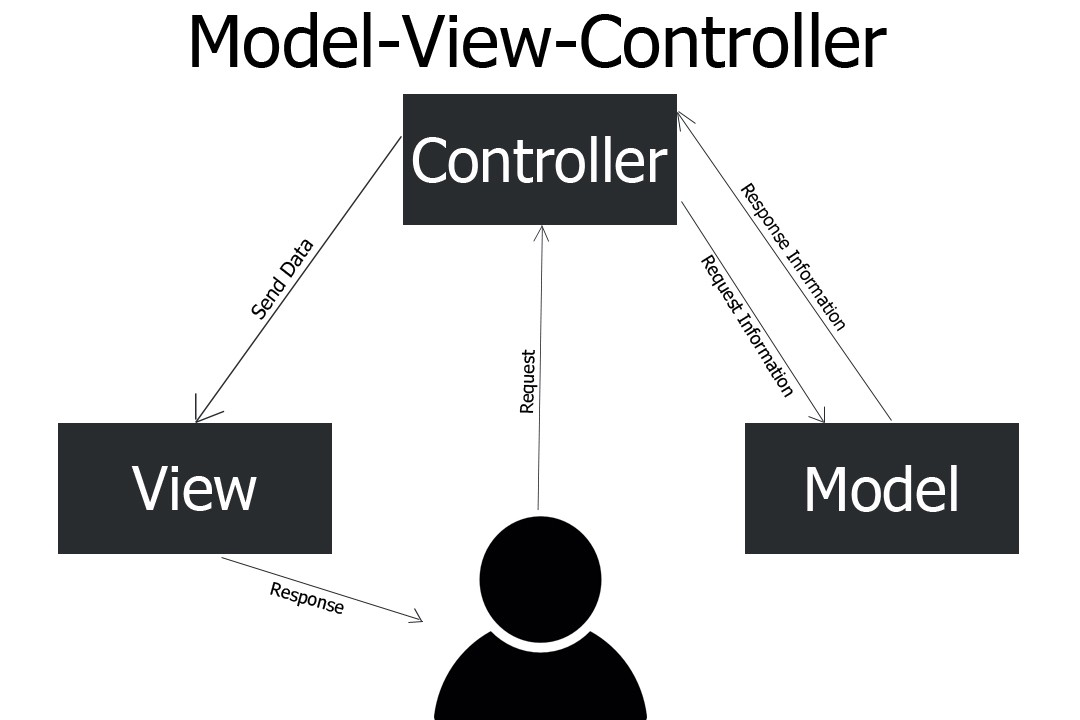
\includegraphics[scale=0.25]{assets/mvc.jpg}
      \caption{Model View Controller}
      \label{fig:mvc}
\end{figure}
% %%%%%%%
%%%%
%%%%

\subsection{Codebase Architecture}
Monolithic applications fit best for use cases where the requirements are pretty simple, the app is expected to handle a limited amount of traffic. 

If all the functionalities of a project exist in a single codebase, then that application is known as a monolithic application. We all must have designed a monolithic application in our lives in which we were given a problem statement and were asked to design a system with various functionalities. We design our application in various layers like presentation, service, and persistence and then deploy that codebase as a single jar/war file. This is nothing but a monolithic application where “mono” represents the single codebase containing all the required functionalities.
\begin{figure}[!ht]
      \center
      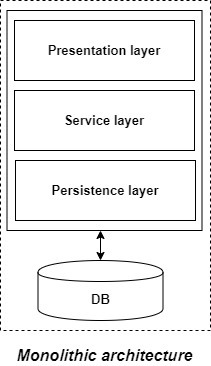
\includegraphics[scale=0.50]{assets/monolithic.jpg}
      \caption{Monolithic Applications}
      \label{fig:monoapp}
\end{figure}

% Disadvantages of Monolithic applications:
% \begin{enumerate}
%       \item
%       It becomes too large with time and hence, difficult to manage.
%       \item
%       We need to redeploy the whole application even for a small change.
%       \item
%       As the size of the application increases, its start-up and deployment time also increases.
%       \item
%       For any new developer joining the project, it is very difficult to understand the logic of a large Monolithic application even if his responsibility is related to a single functionality.
%       \item
%       Even if a single part of the application is facing a large load/traffic, we need to deploy the instances of the whole application in multiple servers. It is very inefficient and takes up more resources unnecessarily. Hence, horizontal scaling is not feasible in monolithic applications.
%       \item
%       It is very difficult to adopt any new technology which is well suited for a particular functionality as it affects the whole application, both in terms of time and cost.
%       \item
%       It is not very reliable as a single bug in any module can bring down the whole monolithic application.
% \end{enumerate}
% Advantages of monolithic applications:
% \begin{enumerate}
%       \item
%       Simple to develop relative to microservices where skilled developers are required in order to identify and develop the services.
%       \item
%       Easier to deploy as only a single jar/war file is deployed.
%       \item
%             Relatively easier and simple to develop in comparison to microservices architecture.
%       \item
%             The problems of network latency and security are relatively less in comparison to microservices architecture.
%       \end{enumerate}

\subsection{Controller Architecture}
REpresentational State Transfer \ac{REST}, is an architectural style for providing standards between computer systems on the web, making it easier for systems to communicate with each other. REST-compliant systems, often called RESTful systems, are characterized by how they are stateless and separate the concerns of client and server.

\subsection{Cloud Architecture}
      \ac{SaaS} , which allows us to set up services, such as application servers and databases, as needed to create the apps we need. This type of system typically works in a cloud or hybrid cloud environment, which often makes provisioning of servers and software as simple as entering some configurations and clicking a button.
      
      This type of setup is perfect for the MEAN stack in the deployment stage, as each piece of the MEAN stack is easily placed into the cloud and thus can be easily provisioned, so they are widely available on PaaS services and can be used quickly when needed.
      %%%
      
\section{Frameworks}
\subsection*{MEAN stack}
While the name sounds like “mean”, it stands for the software pieces that are used to create a particular development stack: MongoDB, ExpressJS, Angular, and NodeJS. One of the biggest advantages of using this particular development stack is the ability to allow developers to use one consistent data model across the stack, using \ac{JSON} and BSON (for MongoDB). This allows for quick transitions between the various pieces of the stack, especially when a single programmer has to handle more than one portion of the stack.

\begin{figure}[!ht]
      \center
      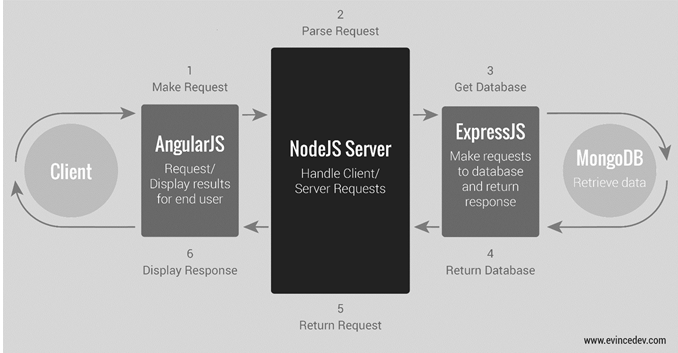
\includegraphics[scale=0.50]{assets/meanphases.png}
      \caption{The Flow In Mean Stack}
      \label{fig:mean}
\end{figure}
\begin{enumerate}
      \item 
      When a client makes any request, it is firstly processed by the Angular.
      \item 
      After that, the Request enters phase 2 which is NodeJS.
      \item 
      After that Request enters phase 3, and ExpressJs it send a request to the database.
      \item 
      After that, MongoDB retrieves the data and return the response to the ExpressJs.
      \item 
      Then ExpressJs return response to the NodeJS and then NodeJS return it to the AngularJS to display the result.
\end{enumerate}

\begin{figure}[H]
      \center
      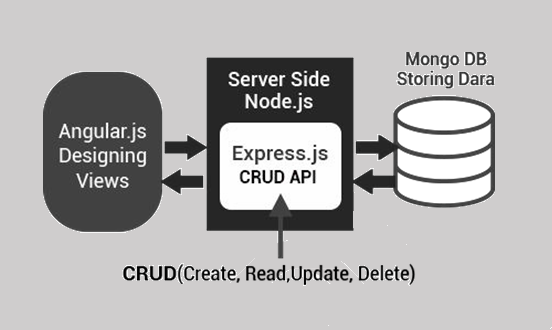
\includegraphics[scale=0.55]{assets/meanarchdesc.png}
      \caption{Communication In Mean Stack}
      \label{fig:mean}
\end{figure}

\begin{itemize}
      \item 
      Create (POST) Make something
      \item 
      Read (GET) Get something
      \item 
      Update (PUT) Change something
      \item 
      Delete (DELETE) Remove something
\end{itemize}




\subsection{Front-End}
\subsubsection{Single Page Application}
Single-page application \ac{SPA} is an app that works inside a browser and does not require page reloading during use.
SPAs are all about serving an outstanding UX by trying to imitate a “natural” environment in the browser, no page reloads, no extra wait time. It is just one web page that you visit which then loads all other content using JavaScript, which they heavily depend on.
SPA requests the markup and data independently and renders pages straight in the browser.
Single-page sites help keep the user in one, comfortable web space where content is presented to the user in a simple, easy, and workable fashion.
% \paragraph*{Pros}
% \begin{enumerate}
%       \item 
%       SPA is fast, as most resources (HTML+CSS+Scripts) are only loaded once throughout the lifespan of the application. Only data is transmitted back and forth.
%       \item 
%       The development is simplified and streamlined. There is no need to write code to render pages on the server.
%       \item 
%       SPAs are easy to debug with Chrome, as you can monitor network operations, investigate page elements and data associated with it.
%       \item 
%       It’s easier to make a mobile application because the developer can reuse the same backend code for web applications and native mobile applications.
%       \item 
%       SPA can cache any local storage effectively. An application sends only one request, store all data, then it can use this data and works even offline.
% \end{enumerate}
\subsubsection{Angular 9}
Angular is an app-design framework and development platform for creating efficient and sophisticated single-page apps in \ac{HTML}, \ac{CSS}, and Typescript which is a superset of JavaScript. Angular provides built-in features for animation, \ac{HTTP} service, and materials which in turn have features such as auto-complete, navigation, toolbar, menus, etc.

\subsection{Back-End}

\subsubsection{Node Js}
Node.js is open-source, and a cross-platform runtime environment for developing server-side and networking applications. Node.js applications are written in JavaScript, and can be run within the Node.js runtime on OS X, Microsoft Windows, and Linux.
Node.js also provides a rich library of various JavaScript modules which simplifies the development of web applications using Node.js to a great extent.

The following are some of the important features that make Node.js the first choice of software architects.
\begin{enumerate}
      \item
            Asynchronous and Event-Driven
            %  All APIs of Node.js library are asynchronous, that is, non-blocking. It essentially means a Node.js based server never waits for an API to return data. The server moves to the next API after calling it and a notification mechanism of Events of Node.js helps the server to get a response from the previous API call.
      \item
            Very Fast
            %  Being built on Google Chrome's V8 JavaScript Engine, Node.js library is very fast in code execution.
      \item
            Single-Threaded but Highly Scalable
            %  Node.js uses a single-threaded model with event looping. The event mechanism helps the server to respond in a non-blocking way and makes the server highly scalable as opposed to traditional servers which create limited threads to handle requests. Node.js uses a single-threaded program and the same program can provide service to a much larger number of requests than traditional servers like Apache HTTP Server.
      \item
            No Buffering
            %  Node.js applications never buffer any data. These applications simply output the data in chunks.
      \item
            Node.js is released under the MIT license
\end{enumerate}



\subsubsection{Express Js}
ExpressJS is a web application framework that provides us with a simple API to build websites, web apps, and back ends. With ExpressJS, we need not worry about low-level protocols, processes, etc.
Express provides a minimal interface to build our applications. It provides us the tools that are required to build our app. It is flexible as there are numerous modules available on npm, which can be directly plugged into Express.
Express was developed by TJ Holowaychuk and is maintained by the Node.js Foundation and numerous open source contributors.



\subsubsection{MongoDB}
MongoDB is a cross-platform, document-oriented database that provides, high performance, high availability, and easy scalability. MongoDB works on the concept of collection and document.
\begin{enumerate}
      \item
            Database:
            The database is a physical container for collections. Each database gets its own set of files on the file system. A single MongoDB server typically has multiple databases.
      \item
            Collection:
            A collection is a group of MongoDB documents. It is the equivalent of an RDBMS table. A collection exists within a single database. Collections do not enforce a schema. Documents within a collection can have different fields. Typically, all documents in a collection are of similar or related purposes.
      \item
            Document:
            A document is a set of key-value pairs. Documents have a dynamic schema. Dynamic schema means that documents in the same collection do not need to have the same set of fields or structures, and common fields in a collection's documents may hold different types of data.
\end{enumerate}


\subsubsection{Mongoose}
Mongoose is an Object Data Modeling \ac{ODM} library for MongoDB and Node.js. It manages relationships between data, provides schema validation, and is used to translate between objects in code and the representation of those objects in MongoDB.





% section
% section
% section





\section{Programming Languages}

\subsection{Conception}
\paragraph*{PlantUML}
PlantUML is an open-source tool allowing users to create \ac{UML} diagrams from a plain text language. The language of PlantUML is an example of a Domain-specific language. It uses Graphviz software to lay out its diagrams. 
\subsection{General}
\paragraph*{JavaScript Object Notation}
\ac{JSON} is a lightweight data-interchange format. It is easy for humans to read and write. It is easy for machines to parse and generate. It is based on a subset of the JavaScript Programming Language Standard ECMA-262 3rd Edition - December 1999. \ac{JSON} is a text format that is completely language independent but uses conventions that are familiar to programmers of the C-family of languages, including C, C++, C\#, Java, JavaScript, Perl, Python, and many others. These properties make \ac{JSON} an ideal data-interchange language.

\subsection{Front-End}
\subsubsection{Typescript}
TypeScript is an open-source programming language developed and maintained by Microsoft. It is a strict syntactical superset of JavaScript and adds optional static typing to the language. TypeScript is designed for the development of large applications and transcompiles to JavaScript. As TypeScript is a superset of JavaScript, existing JavaScript programs are also valid TypeScript programs.

\subsubsection{HTML}
Hypertext Markup Language \ac{HTML} is the standard markup language for documents designed to be displayed in a web browser. It can be assisted by technologies such as Cascading Style Sheets (CSS) and scripting languages such as JavaScript.

% Web browsers receive HTML documents from a web server or local storage and render the documents into multimedia web pages. HTML describes the structure of a web page semantically and originally included cues for the appearance of the document.



\subsubsection{CSS}
Cascading Style Sheets \ac{CSS} is a style sheet language used for describing the presentation of a document written in a markup language like HTML. CSS is a cornerstone technology of the World Wide Web, alongside HTML and JavaScript.

% \ac{CSS} is designed to enable the separation of presentation and content, including layout, colors, and fonts. This separation can improve content accessibility, provide more flexibility and control in the specification of presentation characteristics, enable multiple web pages to share formatting by specifying the relevant CSS in a separate .css file, and reduce complexity and repetition in the structural content.


\subsection{Back-End}
\subsubsection{Javascript}
JavaScript often abbreviated as JS, is a programming language that conforms to the ECMAScript specification. JavaScript is high-level, often just-in-time compiled, and multi-paradigm. It has curly-bracket syntax, dynamic typing, prototype-based object-orientation, and first-class functions.


% section
% section
% section





